% Metódy inžinierskej práce

\documentclass[10pt,oneside,english,a4paper]{article}

\usepackage[english]{babel}
%\usepackage[T1]{fontenc}
\usepackage[IL2]{fontenc} % lepšia sadzba písmena Ľ než v T1
\usepackage[utf8]{inputenc}
\usepackage{graphicx}
\usepackage{booktabs} 
\usepackage{caption} 
\usepackage{subcaption} 
\usepackage{multicol}
\usepackage{amsmath, amssymb}
\usepackage{geometry}
\usepackage{array, hhline}
\usepackage{cite}
\usepackage[normalem]{ulem}
\usepackage[shortlabels]{enumitem}
\usepackage{comment}
\usepackage{indentfirst}
\usepackage{titlesec}
\usepackage{tabularx}
\usepackage{url} % príkaz \url na formátovanie URL
\usepackage{hyperref} % odkazy v texte budú aktívne (pri niektorých triedach dokumentov spôsobuje posun textu)


%\usepackage{times}


\pagestyle{headings}

\title{Real-time data processing in autnomous vehicles\thanks{Semestrálny projekt v predmete Metódy inžinierskej práce, ak. rok 2023/24, vedenie: Pavol Baťalík}} % meno a priezvisko vyučujúceho na cvičeniach

\author{Maksim Alehash\\[2pt]
	{\small Slovenská technická univerzita v Bratislave}\\
	{\small Fakulta informatiky a informačných technológií}\\
	{\small \texttt{xalehash@stuba.sk}}
	}

\date{\small\today} % upravte

\titleformat*{\section}{\large\bfseries}
\titleformat*{\subsection}{\bfseries}
\titleformat*{\subsubsection}{\itshape}

\begin{document}

\maketitle

\begin{abstract}
The astounding leaps in AI technology have made AVs a great variant for modern transportation. Key elements that they hold are the prioritization of passengers' safety, adaptation to the comfort of the passengers and making the ride as efficient as possible. These are the things that every self-driven vehicle should include and hold up to. In order to get the optimal results in the shortest amount of time possible, the machines need to make split-second decisions in order to achieve them while at the same time not depending on human action. 
\par The article provides a comprehensive exploration of the critical role of real-time data processing, which is one of the most crucial parts of AVs. It covers the essence and the functioning of many cutting-edge technologies and methods that are being used, outlining general data processing procedures and touches on the safety and comforts whilst travelling around places, but also the potential risks and challenges it can pose. Ultimately, the article illustrates to readers the intricacies and implications of real-time data processing that play a crucial role in AVs.

\end{abstract}

\newpage\section{Introduction}

\indent Although AV are quite a recent technological invention in today's rapidly evolving world of transportation, they have certainly reshaped the way we see the future of mobility and innovation. At the core of this revolutionary technology lies the capability to instantaneously perceive, analyze and respond to a dynamic and complex environment in real-time, all without the need for human intervention. 
\par This article provides a comprehensive overview of the critical importance of real-time data processing in AVs. We begin with the role and significance of sensors. 
Then we head to various algorithms that are used within AVs. Then we discuss the architecture of data processing used in AVs. Then we discuss how data processing contributes to the safety of AVs and the prevention of accidents and threats. Finally, we emphasize on the future of AVs and analyze upcoming trends and research direction.

%nova sekcia

\section{Sensors} \label{sensors}

\indent The central part to the success of AV is their ability to understand and interpret their surroundings without any mistakes. They are equipped with an array of internal and external sensors which help the vehicle function autonomously while storing a tremendous volume of data. Here we list the most important sensors:

\begin{figure*}[!h]
\centering
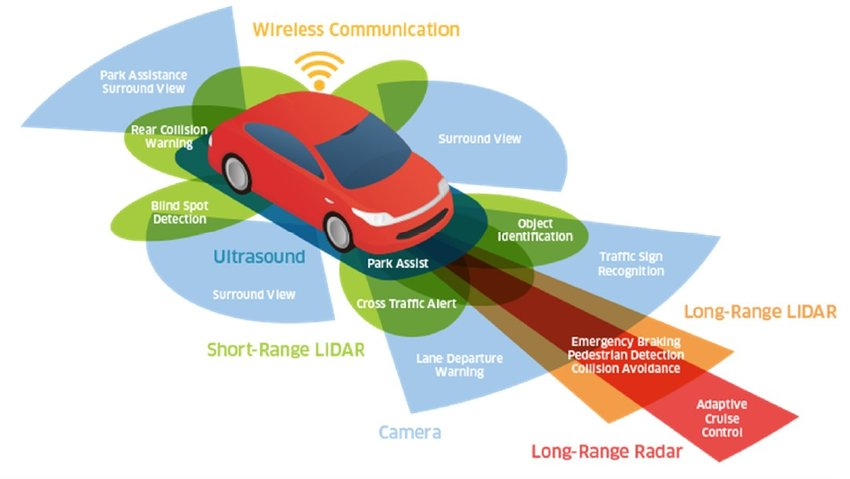
\includegraphics[scale=0.4]{SensorsScheme.png}
\caption{Sensors coverage diagram for an autonomous vehicle}
{Source: \url{https://www.researchgate.net/figure/Sensors-coverage-diagram-for-an-autonomous-vehicle-taken-from-6_fig1_351407935}}
\label{fig:p_sensors}
\end{figure*}


\subsection{Cameras}
\par Cameras can be perceived as the most basic type of sensors. Its role is to detect objects such as lanes, traffic signs and lights, and pedestrians to name a few. They provide readily interpretable 2D visual data that can span from a few centimetres to up to 100 meters. Images captured by cameras consist of pixels. Each pixel in an image collectively contributes to an array of pixels that form the entire image. The amount of data output generated by cameras is about 20-40 MB/s on average.

\subsection{Radio Detection and Ranging}
\par Radar is the ultimate barrier for obstacle detection. Its primary role is to immediately react to a detected object within a dangerously close range and avoid the impending obstacle or stop the vehicle. They use electromagnetic waves to detect the distance, speed, and angle of objects in the environment. We divide them into short-range, medium-range, and long-range radars, each having different applications and performance. Their range spans from 70m to 200m, depending on the radar itself, and usually produces only 10-100KB of data per second. 

\subsection{Light Detection and Ranging}
\par LiDAR is quite similar to radar, but instead of electromagnetic waves, it uses lasers to precisely measure distance, monitor static and dynamic environments and is used for mapping. Its primary role is to provide precise information for immediate decision-making, allowing the vehicle to navigate and avoid obstacles effectively. By using laser beams, it assesses the brightness of targets and by receiving light pulses back, it creates a high-definition 360-degree 3D map of the surrounding area. The distance range can vary from several centimetres to up to 200 m, depending on the LiDAR itself. Just like radar, it can be divided into short-range, medium-range and long-range LiDARs. It generates around 10-70 MB of data per second, which places a heavy processing load on the system

\subsection{Ultrasonic sensors}
\par Ultrasonic sensors utilize high-frequency sound waves that measure the distance to the vehicle or an object. Their role is to provide accurate distance information in short-range scenarios, particularly for parking assistance and collision avoidance. Thus, short-range ultrasonic sensors with 20m detection range are employed for this reason. Data generation is similar to radar, at around 10-100 KB/s.

\subsection{Global Positioning System}
\par Besides perception, navigation and guidance are essential for an autonomous vehicle. GPS offers comprehensive navigation features that play a crucial role in creating a time-based route from the current position to the destination. The system must adapt to sudden path changes in order to follow the given route. It's praised for its accuracy and adaptability since it continuously redirects its route when unforeseen events, like roadblocks, are present. In many cases where GPS is not that effective, like tunnels, In such scenarios, inertial guidance using gyroscopes and accelerometers (IMU) can be a substitution for GPS.
\cite{functionalarch, computerarch, stateoftheart, Sensorfusion, AIandIoT}

\begin{figure*}[!h]
\centering
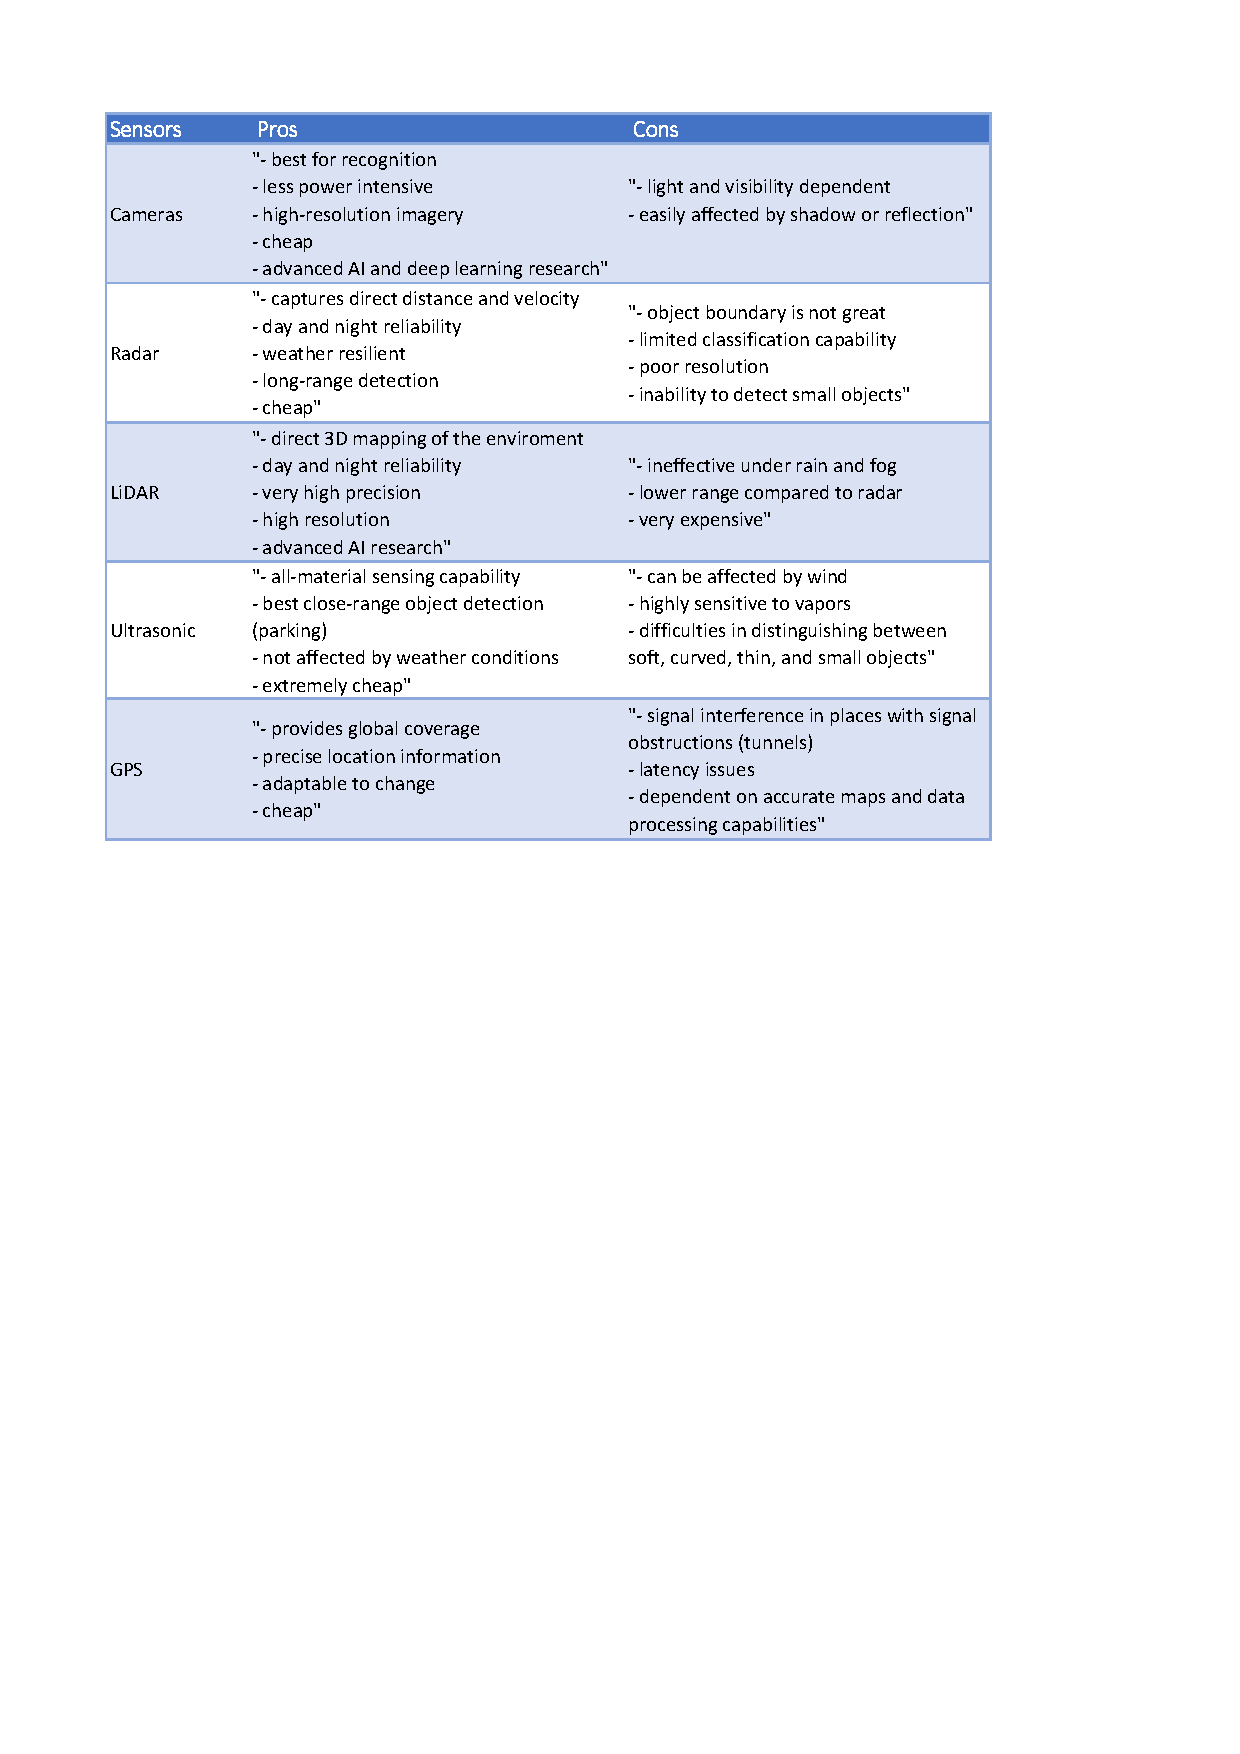
\includegraphics[scale=0.4]{tabulka.pdf}
\caption{Advantages and disadvantages of sensors}
{Source: Microsoft Excel}
{Autor: Maksim Alehash}
\label{fig:p_tabulka}
\end{figure*}

%nova sekcia

\section{Algorithms and techniques of data processing} \label{algorithms}
In the previous section, we talked about the most important sensors of AVs. The ability to process and interpret data in real-time is crucial for any AV. Hence, the true power behind these sensors comes from the algorithms that are implemented into them and the AVs in general.  

\subsection{Artificial intelligence approaches}
\begin{enumerate}[A)]
    \item \textbf{Machine learning}
    \par Machine learning stands at the forefront of innovation by creating and automating analytical models and algorithms. It enhances the system performance for specific tasks by drawing various methods and approaches to uncover hidden insights within data.
    \par We divide it into 3 subfields:
    \begin{itemize}
        \item \textbf{Unsupervised learning} - involves interpreting data based on input information with no defined labels, also known as clustering
        \item \textbf{Supervised learning} - involves training on labelled data based on input and output data
        \item \textbf{Reinforcement learning} - relies on time-delayed and incomplete feedback to shape future decisions
    \end{itemize}
    
    \item \textbf{Deep learning}
    \par In comparison to machine learning, deep learning stands out by autonomously learning high-level features incrementally, utilizing extensive neural network layers with numerous processing units to handle extensive sensory data and facilitating well-informed decision-making.
    \par We can divide it into 3 applications:
    \begin{itemize}
        \item \textbf{Driver profiling} - utilizes time-series data taken from driver's responses in situations in order to enhance the overall quality of autonomous driving
        \item \textbf{Image recognition} - collects and categorizes diverse features from the environment, like lane following and understanding of the environment
        \item \textbf{Object detection} - locates specific objects within collected images and allows them to make corresponding actions, like navigation, and collision avoidance \cite{AIandIoT, Fundamentals, researchresults, Taskoffloading}
    \end{itemize}
\end{enumerate} 

\subsection{Algorithms}
\par Since we've discussed how the sensory part of an AV works, we need to take a closer look at how the vehicle perceives and makes decisions about its tasks. Here we list the most important ones:
\begin{enumerate}[A)]
    \item \textbf{Mapping}
    \par Mapping is the process of the AV collecting data from its surroundings and creating either an image (2D) or point-cloud (3D) map of it.
    \par We can divide mapping into 3 modules based on its surroundings.
    \begin{itemize}
        \item \textbf{Mapping of objects} - this module compiles data received from sensors, mainly camera, radar, and LiDAR, and integrates the received information to create a 2D map
        \item \textbf{Mapping of the road} - this module utilizes images to establish and update the 2D map to describe the road and non-drivable surroundings
        \item \textbf{Mapping traffic of regulations} - this module gathers information to create a 3D map from a LiDAR containing traffic signs, road markings and the positions of traffic lights.  
    \end{itemize}
    
    \item \textbf{Localization}
    \par Localization requires the integration of data gathered from various sensors, mainly GPS and LiDAR, in order to generate a high-precision map and transfer the collected data to pinpoint the precise location of the vehicles. AVs can link sensor measurements together with map data for greater accuracy, which is great for the urban environment.

    \item \textbf{Object detection and tracking} 
    \par Object detection focuses on identifying vehicles, pedestrians, traffic signals/lights, and so on. It's primarily concentrated on moving objects. The integration of LiDAR with sensor fusion enhances 3D environmental understanding. The combination of a 3D map with the vehicle's position enables targeted processing which reduces both processing time and the probability of false detections.
    \par Object tracking is centred on automatically tracking dynamic objects and ensuring safe vehicle operation. For tracking, LiDAR is primarily used since it has the ability of a 360-degree vision and monitor objects over large distances in great detail while tracking every move on the road.

    \item \textbf{Decision-making}
    \par Decision-making combines all of the aforementioned algorithms to formulate a plan in order to input its driving decisions.
    \par We divide it into 3 tasks:
    \begin{itemize}
        \item \textbf{Prediction} 
        \par To ensure the safe navigation of the vehicle in complex scenarios, AVs must possess the capability to anticipate and predict the actions of other drivers and pedestrians. One method involves modelling other vehicles' positions and making probability distributions. Therefore, AVs need perfect information about their surroundings with minimal delays.
        \item \textbf{Path planning} -
        \par The path planning control strategy revolves around the task of determining a geometric path from an initial configuration to the target one in the safest and most convenient way possible. It integrates extensive data, continuously learns and adapts for refined path planning, improving decision-making.
 
        \item \textbf{Obstacle avoidance} 
        \par This algorithm operates on two levels of obstacle avoidance. The first one is the proactive mechanism which calculates certain parameters, like time to collision or predicted minimum distance, which are then adjusted to the local path planning. If the proactive mechanism isn't enough, a second level called the reactive mechanism gets activated. It relies on radar data to identify obstacles and avoid them. 
    \end{itemize}
\end{enumerate}

\begin{figure*}[!h]
\centering
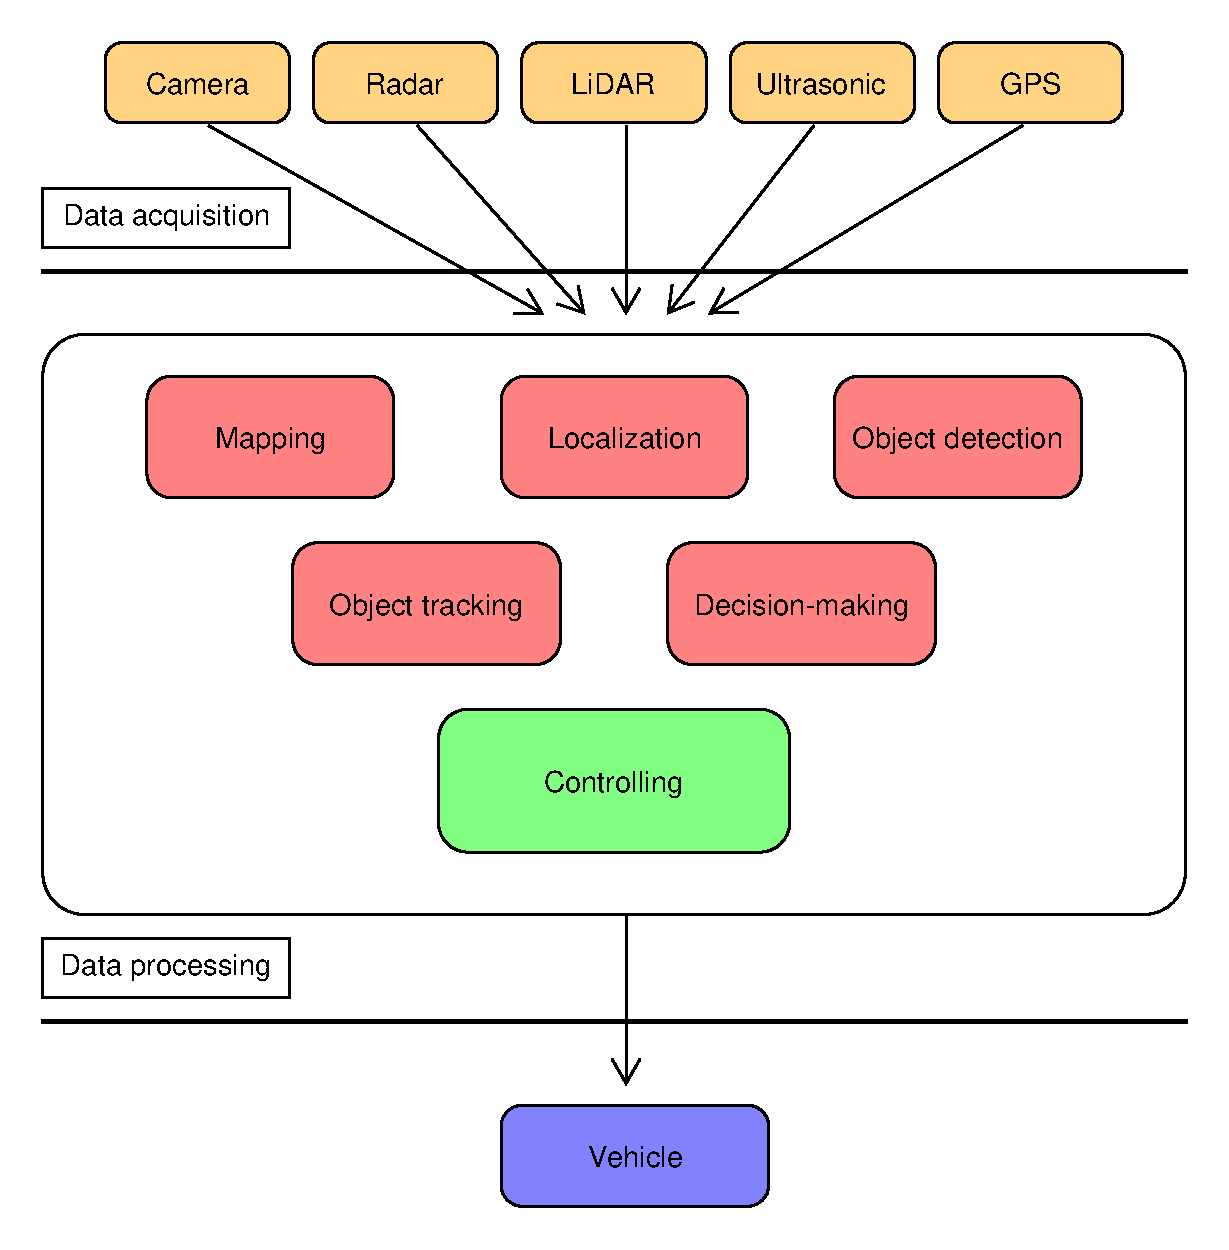
\includegraphics[width=9cm, height=8cm]{algoritmy.pdf}
\caption{Scheme of data acquisition and processing into the vehicle}
{Source: \url{https://www.umlet.com/}}\\
{Author: Maksim Alehash}
\label{fig:p_algoritmy}
\end{figure*}

\par These components collectively form the basis for AVs to navigate through their surroundings and make informed decisions while ensuring the safety and efficiency of their operations. \cite{stateoftheart, functionalarch, approach, computerarch, AIandIoT}

\subsection{Sensor (data) fusion} \label{fusion}
\indent Sensor fusion unites various sensors to create a thorough perspective of the data and combine the information from these sensors. By implementing sensor fusion-based object detection techniques, this method improves precision compared to traditional approaches. With this, it can accurately determine the vehicle's position and orientation. \cite{AIandIoT, Sensorfusion}

%nova sekcia

\section{Data processing architecture} \label{architecture}
Another key component of AV is examining the intricate methods that manage and analyze complex datasets. Here we discuss the difference between cloud and edge computing and vehicular communication. 

\subsection{Cloud vs edge computing}
\begin{enumerate}[A]
    \item \textbf{Cloud computing} 
    \par Cloud computing is a centralized computing model that provides access to a shared pool of necessary computing resources, such as computational power and storage capacity, to process and analyze the massive amounts of data generated by vehicles almost anywhere.
    \par However, the reliance on cloud computing for real-time decision-making in AVs can introduce some limitations such as:
    \begin{itemize}
        \item Reliance on remote data centres introduces latency and hampers quick decision-making
        \item Unreliable internet connections impede data access and application usage
        \item Cloud storage raises concerns about data privacy and security during sensitive information transmission
    \end{itemize}
    
    \item \textbf{Edge computing} 
    \par Edge computing is a decentralized computing model that brings computation and data storage closer to the edge devices, where data is generated. It aims to process data locally, at or near the source, instead of sending it to a centralized cloud server for processing.
    \par Unlike cloud computing, these nearby edge devices allow for reduced latency, improved data transmission utilization, software update and maintenance, and enhanced real-time data analysis capabilities which enable faster response times and reduce the reliance on cloud resources.
    \par Yet, edge computing also faces a few limitations, them being:
    \begin{itemize}
        \item Limited computational and storage resources can lead to compromises in processing capabilities
        \item Deploying, monitoring, and managing edge devices across a bigger network can be more complex
        \item Lack of scalability may limit the ability to handle increasing workloads and adapt to dynamic changes in demand
        \item Data lifetime lasts a few hours or days unlike in cloud-based centers, which is unlimited 
\end{itemize}
\end{enumerate}

\par By combining the strengths of both, we can achieve a comprehensive data processing architecture that balances real-time processing, scalability, and cost efficiency
\cite{understanding, AIandIoT}

\subsection{Vehicular communication}
\textbf{Mobile Edge Computing} 
\par Mobile Edge Computing, or MEC, is a distributed computing architecture that brings computing resources, like processing power and storage, closer to the edge of the network. By doing so it reduces latency, optimizes data processing, and enhances the performance of applications and services in connected environments.

\begin{figure*}[!h]
\centering
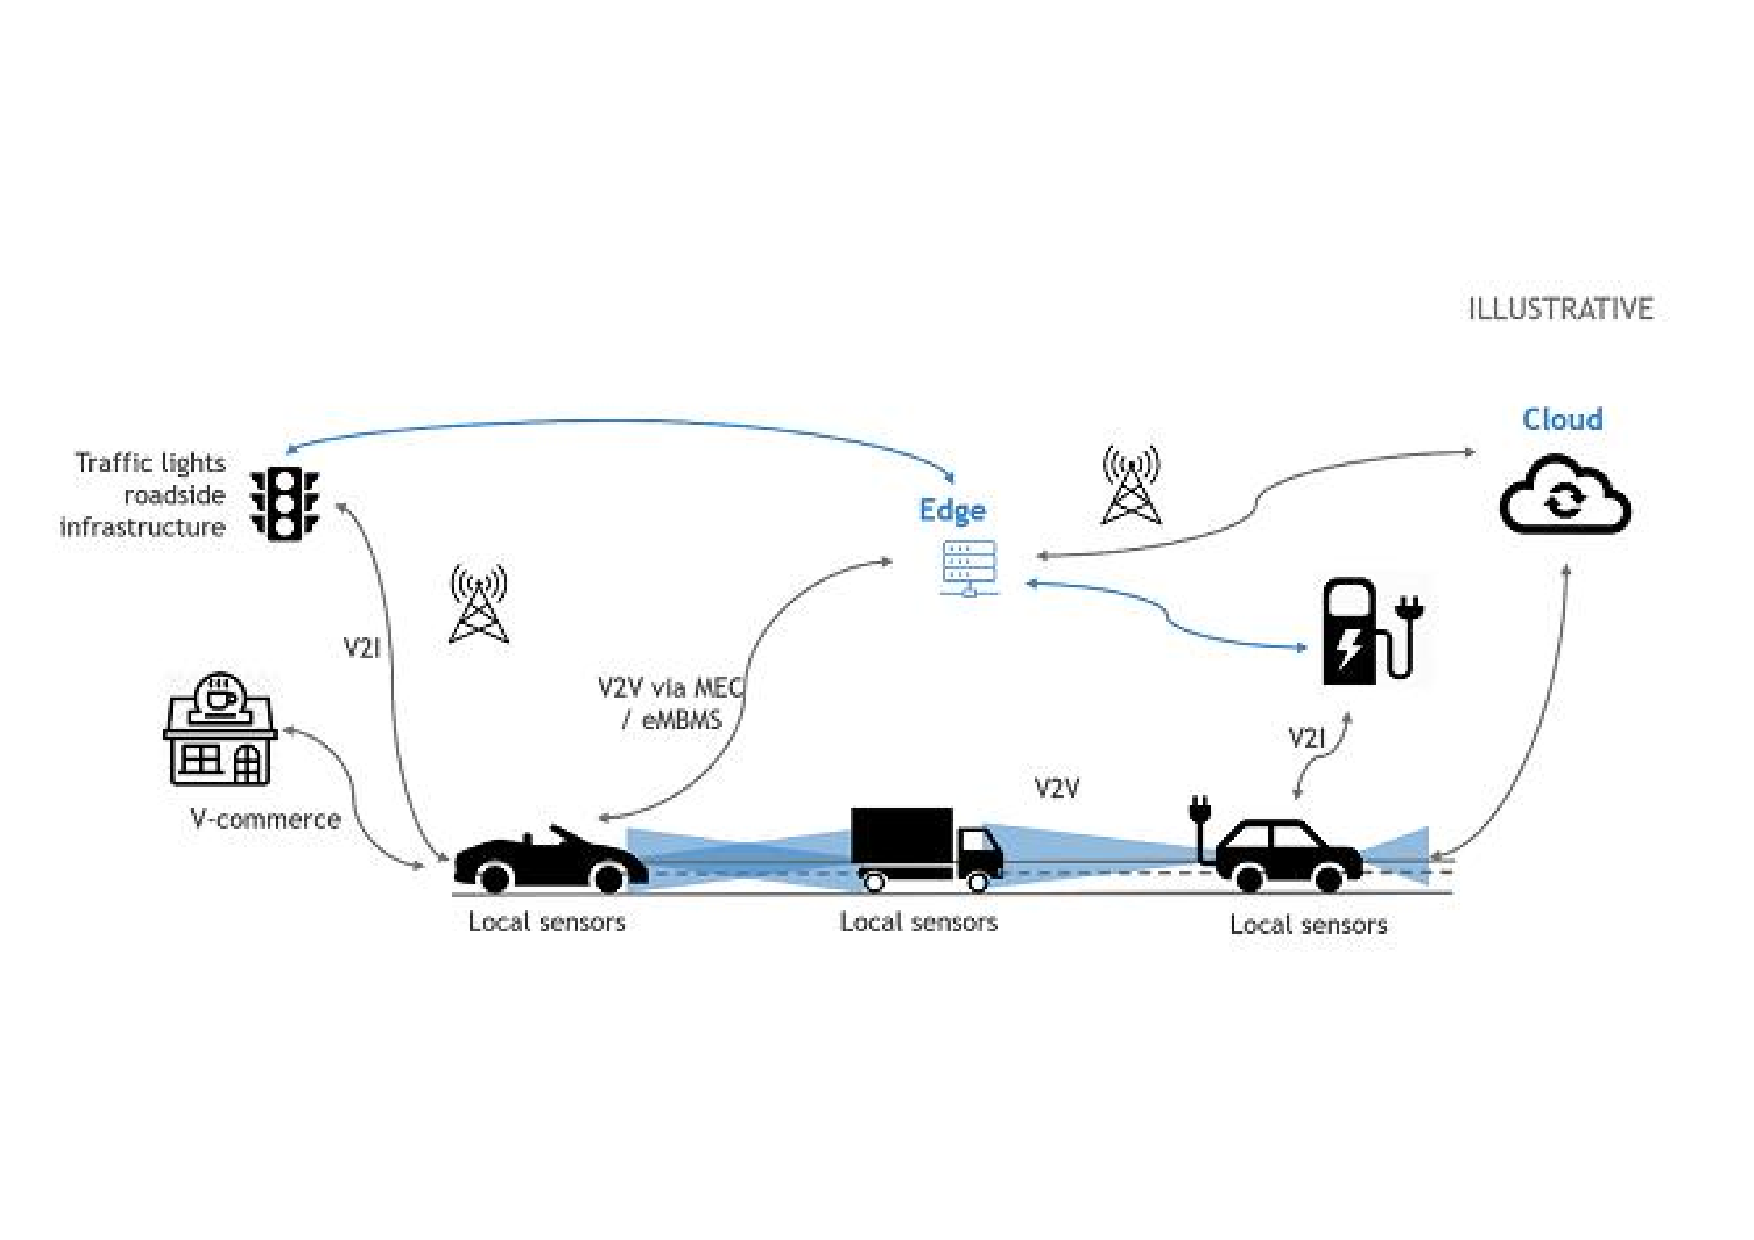
\includegraphics[scale=0.5]{Edgecomputing.pdf}
\caption{Mobile edge computing and vehicle communication}
{Source: \url{https://www.telematicswire.net/connected-vehicles-and-mobile-edge-computing-a-marriage-of-convenience/}}
\label{fig:p_MEC}
\end{figure*}

\par The key component of MEC is the connection of it with V2X (vehicle-to-everything) communication. This comprehensive framework consists of other smaller networks, like V2I, V2P, V2V, and more. Together they create ultra-low latency and high-capacity bandwidth, and enable real-time interactions. MEC's local data processing, edge intelligence, and scalability enhance V2X capabilities, leading to advanced safety features and optimized traffic management. Therefore, they create a strong framework for efficient and intelligent connected vehicles.
\cite{Taskoffloading, understanding}

\subsection{Accelerators}
\par The need for efficient and powerful computing systems becomes essential when it comes to AVs. One crucial component is accelerators. Here we list the most important ones:
\begin{enumerate}
    \item \textbf{Graphics Processing Units}
    \par GPUs are known for their exceptional parallel processing capabilities, making them ideal for computationally intensive tasks, such as image and video processing. They excel at handling sensor data, including camera and LiDAR scans. The parallel architecture of GPUs allows for the execution of multiple tasks at once, leading to faster processing time. However, they consume more power compared to other accelerators, which can be a limitation in the context of energy efficiency.
    \item \textbf{Digital Signal Processors}
    \par DSPs are specialized processors designed to efficiently perform signal processing tasks. They are commonly used for sensor fusion, which we discussed before. DSPs offer high-performance signal processing capabilities while consuming relatively less power compared to GPUs. 
    \item \textbf{Field-Programmable Gate Arrays}
    \par FPGAs are programmable semiconductor devices that can be adjusted for specific tasks, like object detection and tracking. Their re-programmability makes them flexible and suitable for application-specific optimization, but the design and programming are complex and time-consuming, FPGAs are often used for tasks that require low latency and high bandwidth which enables them to process multiple data streams simultaneously while also saving energy.
    \item \textbf{Application-Specific Integrated Circuits}
    \par ASICs are custom-designed integrated circuits used for specific applications. They provide optimized hardware acceleration for critical tasks, such as perception and decision-making. By implementing dedicated circuits for these functions, ASICs offer Unparalleled performance and power efficiency.\cite{edgecomputing, computerarch, researchresults}
\end{enumerate}

%nova sekcia 

\section{Safety measures} \label{safety}
\par AVs are equipped with advanced sensors, AI, and machine learning algorithms to make decisions without human intervention. However, the deployment of them comes with a set of challenges and issues that need to be addressed in order to mitigate potential threats.

\begin{figure*}[!h]
\centering
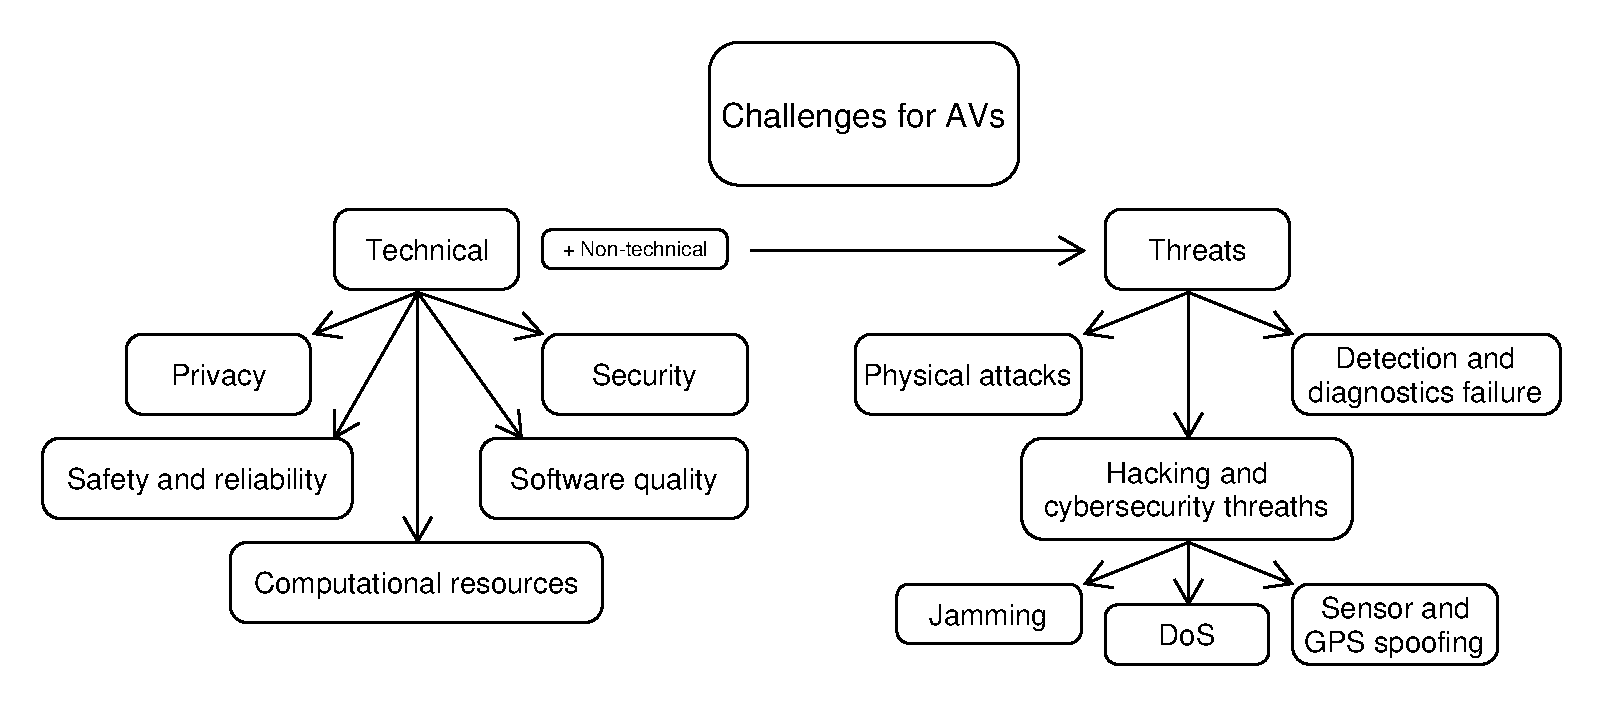
\includegraphics[scale=0.5]{challenges.pdf}
\caption{Challenges facing AVs}
{Source: \url{https://www.umlet.com/}}\\
{Author: Maksim Alehash}
\label{fig:p_challenges}
\end{figure*}

\subsection{Challenges}

\indent \textbf{Technical}
\begin{enumerate}
    \item \textbf{Privacy}
    \par AVs generate a massive amount of data as they collect and process information from their surroundings by sensors, like location, travel routes, and personal preferences. Unauthorized access to this data can lead to privacy breaches and potentially be used for malicious purposes. Implementing access control mechanisms, like robust data encryption and obfuscation to balance information quality with user anonymity, is crucial to protect the privacy of AV users.
    \item \textbf{Security}
    \par AVs are vulnerable to various cyber threats, including hacking attempts and cybersecurity attacks. Malicious actors can exploit vulnerabilities in the vehicle's software or communication systems to gain control or disrupt their operation. Therefore, manufacturers have to take into consideration these measures:
    \begin{itemize}
        \item \textbf{Sensing security} - protecting the integrity of sensors
        \item \textbf{Communication security} - protecting internal and external communication
        \item \textbf{Data security} - preventing data leakage during transmission and storage
        \item \textbf{Control security} - protecting against cyber attacks
    \end{itemize}
    Secure communication protocols, intrusion detection systems, and regular security maintenance are necessary to ensure the safety of AVs.
    \item \textbf{Software quality}
    \par Ensuring software quality in such complex systems is a difficult task. AVs need a good portion of their development budget to go through rigorous testing and validation due to their critical decision-making nature, which can impact human safety. Therefore, they require robust software that can handle various scenarios with minimal errors. In addition, constant software updates and maintenance are important to improve the overall performance of the vehicle.
    \item \textbf{Computational resources}
    \par  A key challenge in Avs is the need for substantial computational resources. The sheer amount of data collected by these sensors requires powerful processors, such as GPUs and FPGAs, and efficient memory management. The limited computational resources on board pose a challenge in terms of real-time data processing and decision-making. 
\end{enumerate}
\indent \textbf{Non-technical}
\par Non-technical challenges include:
\begin{enumerate}
    \item \textbf{Legality and regulations} - legal challenges due to inadequate laws for AVs' unique characteristics 
    \item \textbf{Consumer trust} - widespread adoption relies on public trust and acceptance
    \item \textbf{Infrastructure readiness} - existing infrastructure may not support AVs
    \item \textbf{Ethical concerns} - AVs face moral dilemmas in decision-making
    \item \textbf{Uncertain costs} - financial challenges from both consumers and manufacturers
\end{enumerate}

\subsection{Threats}
\begin{enumerate}
    \item \textbf{Physical attacks}
    \par AVs are susceptible to physical attacks that can compromise their safety and operation. These attacks range from vandalism to intentional collisions. Protecting AVs from them requires measures such as fool-proof designs, secure parking facilities, and surveillance systems.
    \item \textbf{Detection and diagnostics failure}
    \par Sensory systems are responsible for identifying and responding to hazards on the road and their failure can have severe consequences. We can divide them into 3 parts:
    \begin{itemize}
        \item \textbf{Sensor failure} - lack of universal standards for defining sensor failures poses risks in self-driving applications
        \item \textbf{Sensor data failure} - functional sensors may report inaccurate data due to obstruction and deviations 
        \item \textbf{Algorithm failure} - algorithms struggle in challenging lighting or weather conditions to detect road obstacles or lanes
    \end{itemize}
    \item \textbf{Hacking and cybersecurity threats}
    \par AVs are constantly connected to external networks, making them vulnerable to hacking and other cybersecurity threats. Here we list some of the most common ones:
    \begin{itemize}
        \item \textbf{Illusion attack and GPS spoofing attack} - manipulating or compromising sensors to provide incorrect information about the location of the vehicle, causing confusion in the navigation system
        \item \textbf{Denial of Service attack} - overloading the network with irrelevant data to make it unresponsive to genuine users and potentially causing damage to the vehicle, edge stations, or the network
        \item \textbf{Sybil attack} - falsifying the identity of a vehicle or user to disrupt the normal functioning of the network, leading to false information about location, traffic and road conditions, and other events
        \item \textbf{Replay attack} - sending out previously stored messages to deceive other entities on the network into believing past events are occurring again
        \item \textbf{Passive eavesdropping attack} - stealthy attack involving constant monitoring of network traffic to collect information about the network
        \item \textbf{Jamming attack} - disrupting communication channels through signal jamming, creating excessive noise in the network or disrupting communication channels to impact GPS signals and overall network functionality        
    \end{itemize}
\end{enumerate}
\par With these attacks, malicious attackers can exploit vulnerabilities in the vehicle's software or communication protocols to gain unauthorized access or manipulate its behaviour. Therefore, implementing robust cybersecurity measures, like encryption, authentication, and intrusion detection systems, are important to alleviate these threats \cite{researchresults, stateoftheart, Communicationsecurity, edgecomputing}

%nova sekcia 

\section{Future directions} \label{future}
\par The future trajectory of autonomous vehicles is marked by advancements in efficiency, connectivity, safety, and security. These key components are here to reshape the landscape of intelligent transportation and integrate AVs into daily operations.
\par Efficiency assumes a critical role in optimizing the performance of AVs. AI enhancements form the foundation of adaptive intelligence. The ongoing evolution of machine learning algorithms empowers these vehicles to obtain insights from real-world scenarios, continually refining their operational performance and reducing energy consumption. The integration of edge computing further accelerates this process, facilitating localized data processing for rapid decision-making, therefore reducing latency and dependence on external networks.  
\par Connectivity facilitates a sophisticated network of communication between autonomous vehicles and their surrounding. V2X communication enhancements extend the scope of interaction, enabling vehicles to exchange critical information not only amongst themselves but also with smart infrastructure for smoother traffic flow. The integration of 5G connectivity enhances this network, establishing a high-speed, low-latency communication infrastructure that underpins a responsive and dynamic transportation ecosystem.
\par Safety is a primary concern for any industry that specializes in AVs. AI-powered human behaviour prediction enables vehicles to anticipate and respond to the actions of pedestrians and other drivers in order to take appropriate actions to avoid accidents. The implementation of Advanced Driver Assistance Systems (ADAS) increases situational awareness, providing a safety net through features like collision avoidance, emergency braking and lane-keeping assistance. This system will continue to evolve, providing increased levels of automation and assisting drivers in complex traffic scenarios.
\par Security is important given the evergrowing reliance on data. Robust cybersecurity measures are essential, while also encompassing continuous system monitoring, advanced encryption, and secure data transmission. This proactive approach ensures the integrity of vehicles's systems, safeguarding against potential cyber threats such as unauthorized access and interference.
\par These advancements will pave the way for highly efficient, safe, and intelligent Avs that can navigate complex road scenarios with ease.\cite{Communicationsecurity, edgecomputing, stateoftheart, understanding}

%nova sekcia 

\section{Conclusion} \label{conclusion}
\par In conclusion, the integration of real-time data processing in autonomous vehicles represents a pivotal advancement in the evolution of intelligent and modern transportation systems. The collection of cutting-edge technologies, including sophisticated sensors, AI algorithms, and intricate data processing mechanisms, introduces a new era of precision and adaptability for self-driving vehicles. 
\par These components not only enable AVs to navigate through complex and dynamic environments but also lay the foundation for a multitude of advancements that extend beyond the autonomy of AVs. Not only do they strengthen safety measures to protect others but also shaping the emergence of smart cities and an interconnected transportation network. The continuous refinement and integration of these technologies reflect a dynamic trajectory, where ongoing research efforts and innovations converge to redefine the aspects of movement.
\par Looking ahead, real-time data processing in AVs is a transformative force with far-reaching implications beyond current capacities. The ongoing journey of it encompasses not just a technological narrative but also a transformative force in shaping the future of transportation.

%nova sekcia 

\section{Reakcia an témy} 
\par \textbf{Spoločenské súvislosti informatiky} - The integration of AVs into society introduces transformative changes, prompting discussions on safety, the impact on drivers, and the adaptation of traffic systems to these new technologies. Addressing societal acceptance and educating the public about the advantages and safety of AVs becomes pivotal.
\par \textbf{Technológia a ľudia} - As AVs become a reality, there emerge technological challenges and risks for individuals, particularly concerning safety and risk management. Significantly, the question arises of how to educate people to a level where they can comprehend and effectively engage with these emerging technologies.
\par \textbf{Udržateľnosť a etika} - The emergence of AVs holds the potential to enhance sustainability by optimizing transportation systems and reducing emissions. However, ethical considerations come to the forefront, especially in programming vehicles to make decisions during emergencies and navigating value judgments in diverse scenarios. Striking a balance between technological progress and ethical standards is essential.


\newpage
\bibliography{literatura}
\bibliographystyle{abbrv} % prípadne alpha, abbrv alebo hociktorý iný
\end{document}






